\section{Introducción}

El \textbf{aprendizaje automático} es una rama de la inteligencia artifical en la que \textbf{los sistemas son capaces de adquirir conocimiento a partir de datos} \cite{GoodFellowBook}. Se dice que un programa aprende de la experiencia $E$ respecto de alguna tarea $T$ y una medición de rendimiento $P$ si su rendimiento en $T$, medido por $P$, mejora con la experiencia $E$ \cite{mitchell1997machine}. Nos referimos a este programa como modelo. Existen muchos tipos o subramas de aprendizaje automático dependiendo de la naturaleza de esta tarea $T$ y de su medidor de rendimiento $P$. 

El \textbf{entrenamiento de un modelo es el proceso de optimizar sus parámetros} (equivalentemente pesos), es decir, su representación interna; para \textbf{minimizar una función de coste} (equivalentemente función de error o de pérdida) $C$ que mide el error en el rendimiento. El dominio de dicha función es el espacio de valores que pueden tomar los pesos, normalmente representado de forma tensorial; y su imagen es comúnmente un real no negativo. El objetivo principal del entrenamiento es que el modelo sea capaz de aprender los patrones en un conjunto de datos para luego poder generalizarlos en otros que no ha visto previamente. Diremos que existe un sobreajuste cuando se aprenden los patrones específicos de los datos pero luego no se generaliza bien. La estrategia que usamos para optimizar los pesos es llamada algoritmo de aprendizaje.

El \textbf{aprendizaje profundo} es un paradigma del aprendizaje automático en el que los modelos tienen varios niveles de representación obtenidos a través de la composición de módulos sencillos pero comúnmente no lineales, que transforman la representación de los datos sin procesar hacia un nivel de abstracción mayor \cite{lecun2015deep}. Esta rama comenzó a ganar peso en la década de los 2000 y un punto de inflexión fue el resultado de la competición de ImageNet\footnote{\url{http://www.image-net.org/challenges/LSVRC/}} en 2012 \cite{NIPS2012_c399862d}. Actualmente este enfoque es el que mejores resultados consigue, siendo una parte fundamental en la investigación y estructura de las grandes compañías tecnológicas y pudiendo ofrecer aplicaciones comerciales a nivel usuario \cite{Sejnowski18, lecunnDeepForAI}.

\textbf{La mayoría de los modelos en aprendizaje automático se entrenan usando técnicas basadas en el algoritmo de aprendizaje de gradiente descendente} (equivalentemente descenso del gradiente), ya que es la estrategia que mejores resultados ofrece actualmente en cuanto a capacidad de generalización del modelo y rendimiento computacional \cite{GoodFellowBook, CauchyGD}. Ésta se basa en la idea de que puedo moverme hacia puntos de menor valor en la función de error del modelo realizando pequeños movimientos en  sentido contrario a su gradiente como se esquematiza en la Figura \ref{fig:1.GD}, con el objetivo de minimizar el valor de salida. Al tratarse de un algoritmo iterativo, \textbf{es fundamental estudiar su convergencia}, que depende de varios factores y se enfrenta a diversas dificultades, como veremos en secciones posteriores.

El algoritmo de \textbf{\textit{backpropagation} (BP)} permite transmitir la información desde la salida de la función de coste hacia atrás en un modelo con varios módulos de abstracción para así poder \textbf{computar el gradiente de una manera sencilla y eficiente} \cite{rumelbackprop}. Aunque existen otras posibilidades a la hora de realizar éste cómputo, BP es la más usada y extendida gracias a propiedades como su flexibilidad, eficiencia y escalabilidad, que lo hacen destacar por encima de otras opciones \cite{GoodFellowBook}. 

\begin{figure}
    \centering
    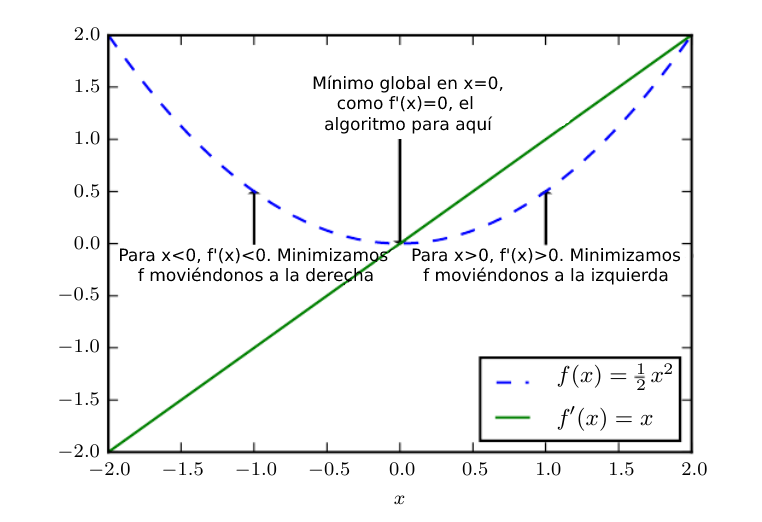
\includegraphics[width=0.75\linewidth]{Plantilla_TFG_latex//imagenes//Mat//1.intro/1.1GDMatIntroGoodFellowBook.png}
    \caption[Ejemplo del proceso de optimización mediante el algoritmo de gradiente descendente]{Ejemplo del proceso de optimización mediante el algoritmo de gradiente descendente aplicado a la función $f(x)=\frac{1}{2}x^2$  (curva azul discontinua). La derivada $f'(x)=x$ (línea verde sólida) indica la pendiente de la función en cada punto. Cuando $x<0$, entonces $f'(x)<0$ y el algoritmo se mueve hacia la derecha para minimizar la función. Cuando $x>0$, entonces $f'(x)>0$ y el algoritmo se mueve hacia la izquierda. El proceso se detiene en $x=0$, que es el mínimo global, ya que en este punto la derivada es cero. Este ejemplo ilustra el principio básico del gradiente descendente: ajustar los parámetros en la dirección opuesta al gradiente para minimizar una función de pérdida. Imagen obtenida y traducida de \cite{GoodFellowBook}}
    \label{fig:1.GD}
\end{figure}



Dependiendo de la familia de modelos que usemos podremos utilizar una estrategia de aprendizaje distinta, como el caso del \textit{Perceptron} y su \textit{Perceptron Learning Algorithm} \cite{patternrecog}. En otros casos como la regresión lineal se usa la estrategia de descenso de gradiente pero el gradiente no tiene por qué calcularse a través de BP. Esto se debe a que en este caso se puede obtener eficientemente a través de librerías matemáticas como \textit{Numpy}\footnote{\url{https://numpy.org/}} en el caso del lenguaje \textit{Python}\footnote{\url{https://es.python.org/}}, ya que esta familia de modelos conlleva menos costo computacional en sus cálculos principalmente debido al escaso número de parámetros en comparación con los de aprendizaje profundo. Para éste sí que es necesario el uso de BP en el caso de que elijamos entrenar mediante gradiente descendente, ya que aunque existen otras alternativas como los métodos numéricos o algunas aproximaciones recientes , no consiguen igualar su rendimiento \cite{EffBackProp, GoodFellowBook, alternativabacknumerical, alternativabackprop1}.


Otra de las características de este algoritmo para el cálculo del gradiente es que los conceptos en los que se basa son simples: optimización, diferenciación, derivadas parciales y regla de la cadena. Lo cual lo convierte a priori en objeto de estudio accesible. En la práctica, los cálculos que se realizan en esta estrategia se implementan a través de la\textbf{ diferenciación automática}, que es una técnica más general que extiende a BP y se usa para el cómputo de derivadas de funciones numéricas de una manera eficiente y precisa \cite{AutomaticDiff}.% Ésta aprovecha el hecho de que cada cálculo que se realiza en un ordenador queda reducido a una secuencia de operaciones aritméticas elementales (suma, resta, multiplicación...) y funciones elementales (exponencial, trigonométricas, ...) para aplicar de forma repetida la regla de la cadena a estos elementos básicos hasta poder obtener derivadas de orden arbitrario. 



\subsection{Motivación}

Tenemos pues que el aprendizaje profundo es el paradigma del aprendizaje automático que mejores resultados obtiene actualmente y más desarrollo e investigación está concentrando, y que basa el entrenamiento (una de las partes fundamentales que determinan el rendimiento del modelo, además de su arquitectura) de los modelos casi por completo en el algoritmo de descenso de gradiente, ya que es el que mejores resultados de generalización y rendimiento ofrece. Éste a su vez depende casi enteramente del algoritmo de BP para calcular el gradiente, ya que aunque existen otras alternativas no son realmente viables. Tanto es así que es muy común la confusión entre este algoritmo y el de gradiente descentente, que se suelen tomar por la misma cosa. Queda así clara la importancia que tiene BP en el campo del aprendizaje profundo y por extensión también al aprendizaje automático. También conviene destacar la cantidad de veces que se utiliza ésta técnica durante el entrenamiento de un modelo. Cada vez que se actualizan los pesos debemos calcular el gradiente, y teniendo en cuenta la duración de los entrenamientos de los modelos más grandes (con mayor número de parámetros), \textbf{el algoritmo de BP puede ser usado miles de veces durante un entrenamiento}.

La eficiencia, escalabilidad y flexibilidad de BP lo han convertido en la opción por defecto para el entrenamiento basado en gradiente descendente para modelos de aprendizaje profundo, sin embargo no hay que olvidar que no se trata de una tarea sencilla: \textbf{la obtención de un mínimo global y la verificación, dado un punto, de que es un mínimo global, se trata de un problema NP-Difícil} generalmente \cite{NPHardProblem}, por lo que se buscan estrategias aproximadas capaces de obtener buenas soluciones en tiempos razonables. Uno de los problemas abiertos en el aprendizaje profundo y en el que influye directamente BP es la reducción computacional del entrenamiento: si se ajustan los pesos en un modelo con un número muy alto de parámetros y usando un conjunto de entrenamiento muy grande (que es una tendencia reciente en aprendizaje profundo), los recursos computacionales pueden resultar insuficientes incluso para las grandes compañías, pudiendo requerir de meses para el  entrenamiento. Por lo que se necesitan algoritmos más escalables y eficientes para afrontarlo \cite{Problem3_accel}.

\textbf{Por ello resulta esencial, mientras no existan alternativas viables, poder ofrecer modificaciones a ambos algoritmos para mejorar sus cualidades}.\textbf{ Atendiendo a la cantidad de uso del algoritmo de BP y su extensión en el campo, una pequeña mejora tendría un alcance enorme}. Sin embargo esta línea de investigación no es muy extensa ya que principalmente se buscan alternativas en lugar de mejoras, pudiendo deberse principalmente a que a priori puede parecer una técnica muy enrevesada y compleja. Veremos en el desarrollo de esta parte que esto no es cierto, y que \textbf{los principios en los que se basa son muy simples}. Es clave comprender su base teórica, funcionamiento e implementación práctica para poder proponer mejoras. 

\textbf{En este contexto, el estudio de la convergencia del algoritmo de gradiente descendente adquiere una relevancia fundamental.} Comprender las condiciones bajo las cuales converge (y en qué medida lo hace hacia soluciones óptimas o subóptimas) permite no solo anticipar su comportamiento en distintos escenarios, sino también diseñar estrategias para mejorar su desempeño. Analizar la convergencia no solo tiene implicaciones teóricas, sino también consecuencias prácticas directas en la eficiencia del entrenamiento, la estabilidad del proceso de optimización y la calidad final del modelo.

\subsection{Objetivos}

El objetivo principal de esta parte matemática es realizar una investigación sobre los algoritmos de descenso de gradiente y BP, proporcionando una visión detallada acerca de los mismos y su implementación. Para ello se divide este objetivo en dos:

\begin{enumerate}
    %\item Exposición de la importancia actual e histórica en el campo del aprendizaje automático y aprendizaje profundo, viendo su estrecha relación con el algoritmo de aprendizaje del gradiente descente.

    
    \item Estudiar de manera teórica el gradiente descendente, haciendo énfasis en su convergencia.

    \item Explorar el uso de BP para el cálculo del gradiente, analizando su implementación a través de la diferenciación automática.

    %\item Analizar de modo teórico las principales variantes del algoritmo de descenso de gradiente. 

 %   \item Realizar una investigación y revisión teórica de las alternativas al cálculo de gradiente basadas en otras estrategias como los métodos numéricos, e inviabilidad de las mismas frente a BP.
\end{enumerate}



